\documentclass{ximera}

\title{How to use Ximera}

\begin{document}
\begin{abstract}
  This course is built in Ximera.
\end{abstract}\maketitle

Mathematics cannot be learned passively: it must be actively
\link[constructed]{http://en.wikipedia.org/wiki/Constructivism_(philosophy_of_education)}
by the person learning it.  This takes time and patience with yourself!
We want you to read this book actively, thinking through each step.

Here are some examples of types of questions we might ask.  Play around 
with them, get them wrong, try the
hints out.  Don't be afraid to fail: \textbf{getting an answer wrong
  never hurts you.}


\begin{example}
  Some problems are multiple-choice:
  \begin{multipleChoice}
    \choice{Don't pick me.}
    \choice{Not me either.}
    \choice[correct]{Pick me!}
    \choice{Also an incorrect choice}
  \end{multipleChoice}
  \begin{feedback}
    Click on the choice that says ``Pick me!''
  \end{feedback}
\end{example}


\begin{example}
  Some problems are select-all that are correct:
  \begin{selectAll}
    \choice{Don't pick me.}
    \choice[correct]{Pick me!}
    \choice[correct]{Pick me too!}
    \choice[correct]{I'm a correct choice too.}
  \end{selectAll}
  \begin{feedback}
    Click on the choices ``Pick me!'' ``Pick me too!'' and ``I'm a correct choice too.''
  \end{feedback}
\end{example}


\begin{example}
    Some problems will ask you to select an option from a drop-down menu. 
    \wordChoice{\choice[correct]{Pick me!}\choice{Don't pick me!}}
\end{example}


\begin{example}
Some problems will ask you to enter numbers. 
  $3\times 2 = \answer{6}$   
  \begin{hint}
    $3 \times 2$ is the number of objects in $3$ groups of $2$ objects
  \end{hint}
  \begin{hint}
    Look at this picture:
    \begin{image}
      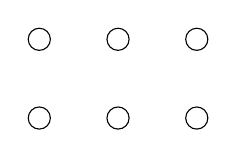
\begin{tikzpicture}
        \draw (0,0) circle (4pt);
        \draw (1,0) circle (4pt);
        \draw (2,0) circle (4pt);
        \draw (0,1) circle (4pt);
        \draw (1,1) circle (4pt);
        \draw (2,1) circle (4pt);
      \end{tikzpicture}
    \end{image}
  \end{hint}
  \begin{hint}
    $3\times 2=6$
  \end{hint}
\end{example}

For this course, you should always have a paper and pencil near at
hand to make notes, doodle pictures, and practice your explanations.
We \textbf{strongly} recommend that you really \textbf{grapple} with 
each example before getting a hint, or moving on.  The difference 
between what you learn by struggling with a problem on your own versus
perusing someone else's solution is astonishing.

With that said, even if you get an answer right you should
\textbf{always} try any hints out afterwards.  They might explain the
concept from a new point of view, or challenge you to think in a
different way.


We support a few different answer types. Here are some example
problems from the different answer types we support:

\begin{example}
Write another expression which has the same answer as $3+1$:
$\answer{4}$
\begin{feedback}
   Try $\verb|5-1|$.
\end{feedback}
\end{example}


\begin{example}
Write a multiplication expression for eight times three.
$\answer{8\times 3}$
\begin{feedback}
   Type $\verb|8*3|$
\end{feedback}
\end{example}


\begin{example}
Write the fraction two thirds.
  $\answer{2/3}$
  \begin{feedback}
    Type $\verb|2/3|$
  \end{feedback}
\end{example}


\begin{example}
Write the mixed-number answer that you get when you do 12 divided by 5.
  $\answer{2+2/5}$
  \begin{feedback}
    Type $\verb|2+2/5|$

    You can also type $\verb|2+(2/5)|$ if you prefer.
  \end{feedback}
\end{example}





\begin{example}
This last one is a little more complicated than we'll usually tackle, 
but try it out to see if you can get it!
  $\frac{x^2+y^2}{7} = \answer{\frac{x^2+y^2}{7}}$
  \begin{feedback}
    Type $\verb|(x^2+y^2)/7|$
  \end{feedback}
\end{example}









As you complete activities the green ``completion bar'' moves at the
top of the page.  This lets you know how close you are to being done
with an activity.

You advance through pages either by completing them and clicking the
``next activity'' button, or by navigating on the little scroll bar at
the top of the page.
 

\end{document}
